\documentclass[12pt,oneside,a4paper]{article}
\usepackage[utf8]{inputenc}
\usepackage[brazil]{babel}

\usepackage{settings/preamble}

\usepackage{listings}

\definecolor{codegreen}{rgb}{0,0.6,0}
\definecolor{codegray}{rgb}{0.5,0.5,0.5}
\definecolor{codepurple}{rgb}{0.58,0,0.82}
\definecolor{backcolour}{rgb}{0.95,0.95,0.92}

\lstdefinestyle{mystyle}{
    language=Scilab,
    backgroundcolor=\color{backcolour},   
    commentstyle=\color{codegreen},
    keywordstyle=\color{magenta},
    numberstyle=\tiny\color{codegray},
    stringstyle=\color{codepurple},
    basicstyle=\ttfamily\footnotesize,
    breakatwhitespace=false,         
    breaklines=true,                 
    captionpos=b,                    
    keepspaces=true,                 
    numbers=left,                    
    numbersep=5pt,                  
    showspaces=false,                
    showstringspaces=false,
    showtabs=false,                  
    tabsize=2,
    literate      =        % Support additional characters
      {á}{{\'a}}1  {é}{{\'e}}1  {í}{{\'i}}1 {ó}{{\'o}}1  {ú}{{\'u}}1
      {Á}{{\'A}}1  {É}{{\'E}}1  {Í}{{\'I}}1 {Ó}{{\'O}}1  {Ú}{{\'U}}1
      {à}{{\`a}}1  {è}{{\`e}}1  {ì}{{\`i}}1 {ò}{{\`o}}1  {ù}{{\`u}}1
      {À}{{\`A}}1  {È}{{\'E}}1  {Ì}{{\`I}}1 {Ò}{{\`O}}1  {Ù}{{\`U}}1
      {ä}{{\"a}}1  {ë}{{\"e}}1  {ï}{{\"i}}1 {ö}{{\"o}}1  {ü}{{\"u}}1
      {Ä}{{\"A}}1  {Ë}{{\"E}}1  {Ï}{{\"I}}1 {Ö}{{\"O}}1  {Ü}{{\"U}}1
      {â}{{\^a}}1  {ê}{{\^e}}1  {î}{{\^i}}1 {ô}{{\^o}}1  {û}{{\^u}}1
      {Â}{{\^A}}1  {Ê}{{\^E}}1  {Î}{{\^I}}1 {Ô}{{\^O}}1  {Û}{{\^U}}1
      {œ}{{\oe}}1  {Œ}{{\OE}}1  {æ}{{\ae}}1 {Æ}{{\AE}}1  {ß}{{\ss}}1
      {ç}{{\c c}}1 {Ç}{{\c C}}1 {ø}{{\o}}1  {å}{{\r a}}1 {Å}{{\r A}}1
      {ã}{{\~a}}1  {õ}{{\~o}}1  {Ã}{{\~A}}1 {Õ}{{\~O}}1
      {ñ}{{\~n}}1  {Ñ}{{\~N}}1  {¿}{{?`}}1  {¡}{{!`}}1
      {°}{{\textdegree}}1 {º}{{\textordmasculine}}1 {ª}{{\textordfeminine}}1
      % ¿ and ¡ are not correctly displayed if inconsolata font is used
      % together with the lstlisting environment. Consider typing code in
      % external files and using \lstinputlisting to display them instead. 
}

\lstset{style=mystyle}

\usepackage{listings}

%\definecolor{codegreen}{rgb}{0,0.6,0}
\definecolor{codegreen}{RGB}{100,174,100}
\definecolor{codegray}{rgb}{0.5,0.5,0.5}
\definecolor{codepurple}{rgb}{0.58,0,0.82}
\definecolor{backcolour}{rgb}{0.95,0.95,0.92}
%\definecolor{backcolour}{RGB}{247,247,242}
%\definecolor{backcolour}{RGB}{252, 252, 247}

\definecolor{codeblue}{RGB}{50,185,185}
\definecolor{stringcolor}{RGB}{188,143,143}
\definecolor{emphcolor}{RGB}{176,24,19}
\definecolor{conditional}{RGB}{160,32,240}
\definecolor{variables}{RGB}{131,67,16}
\definecolor{brackets}{RGB}{74,85,219}
\definecolor{stops}{RGB}{95,158,160}
\definecolor{infinity}{RGB}{218,112,214}
\definecolor{operators}{RGB}{92,92,92}
\definecolor{colon}{RGB}{255,170,0}

\renewcommand{\ttdefault}{pcr}

\lstdefinestyle{scilab_colors}{
    language=Scilab,
    %frame=single,
    backgroundcolor=\color{backcolour},   
    commentstyle=\color{codegreen},
    %keywordstyle=\color{magenta},
    keywordstyle=\color{codeblue},
    numberstyle=\tiny\color{codegray},
    %identifierstyle=\color{blue},
    %stringstyle=\color{codepurple},
    stringstyle=\color{stringcolor},
    basicstyle=\ttfamily\footnotesize,
    emph={function,endfunction},
    emphstyle=\color{emphcolor},
    emph={[2]for, while, if, then, end},
    emphstyle={[2]\color{conditional}},
    emph={[3]lambda, x1, k, n_erro, A, x0, epsilon, alpha, M},
    emphstyle={[3]\bfseries\color{variables}}, 
    emph={[4]\$},
    emphstyle={[4]\color{colon}},
    emph={[5]Metodo_Potencia, Metodo_Potencia_2, Potencia_deslocada_inversa, Potencia_deslocada_Rayleigh},
    emphstyle={[5]\underbar},
    emph={[6]break, continue, return},
    emphstyle={[6]\color{stops}},
    emph={[7]\%inf},
    emphstyle={[7]\color{infinity}},
    emph={[8]Resolve_com_LU},
    emphstyle={[8]\bfseries\color{codepurple}},
    breakatwhitespace=false,         
    breaklines=true,                 
    captionpos=b,                    
    keepspaces=true,                 
    numbers=left,                    
    numbersep=5pt,                  
    showspaces=false,                
    showstringspaces=false,
    showtabs=false,                  
    tabsize=2,
    literate      =        % Support additional characters
      {á}{{\'a}}1  {é}{{\'e}}1  {í}{{\'i}}1 {ó}{{\'o}}1  {ú}{{\'u}}1
      {Á}{{\'A}}1  {É}{{\'E}}1  {Í}{{\'I}}1 {Ó}{{\'O}}1  {Ú}{{\'U}}1
      {à}{{\`a}}1  {è}{{\`e}}1  {ì}{{\`i}}1 {ò}{{\`o}}1  {ù}{{\`u}}1
      {À}{{\`A}}1  {È}{{\'E}}1  {Ì}{{\`I}}1 {Ò}{{\`O}}1  {Ù}{{\`U}}1
      {ä}{{\"a}}1  {ë}{{\"e}}1  {ï}{{\"i}}1 {ö}{{\"o}}1  {ü}{{\"u}}1
      {Ä}{{\"A}}1  {Ë}{{\"E}}1  {Ï}{{\"I}}1 {Ö}{{\"O}}1  {Ü}{{\"U}}1
      {â}{{\^a}}1  {ê}{{\^e}}1  {î}{{\^i}}1 {ô}{{\^o}}1  {û}{{\^u}}1
      {Â}{{\^A}}1  {Ê}{{\^E}}1  {Î}{{\^I}}1 {Ô}{{\^O}}1  {Û}{{\^U}}1
      {œ}{{\oe}}1  {Œ}{{\OE}}1  {æ}{{\ae}}1 {Æ}{{\AE}}1  {ß}{{\ss}}1
      {ç}{{\c c}}1 {Ç}{{\c C}}1 {ø}{{\o}}1  {å}{{\r a}}1 {Å}{{\r A}}1
      {ã}{{\~a}}1  {õ}{{\~o}}1  {Ã}{{\~A}}1 {Õ}{{\~O}}1
      {ñ}{{\~n}}1  {Ñ}{{\~N}}1  {¿}{{?`}}1  {¡}{{!`}}1 {[}{{\textcolor{brackets}{[}}}{1}
        {]}{{\textcolor{brackets}{]}}}{1}
        {(}{{\textcolor{brackets}{(}}}{1}
        {)}{{\textcolor{brackets}{)}}}{1} 
        {+}{{{\color{operators}+}}}1
        {-}{{{\color{operators}-}}}1
        {*}{{{\color{operators}*}}}1
        {/\ }{{{\color{operators}/}}}1
        {=}{{{\color{operators}=}}}1
        {^}{{{\color{operators}\textasciicircum}}}1
        {<}{{{\color{operators}<}}}1
        {>}{{{\color{operators}>}}}1
        %{&}{{{\color{operators}\&}}}1
        %{!=}{{{\color{codegreen}$\neq$}}}1
        %{~}{{{\color{operators}\textasciitilde}}}{1}
        %{:}{{{\color{colon}:}}}{1}
      {°}{{\textdegree}}1 {º}{{\textordmasculine}}1 {ª}{{\textordfeminine}}1
      % ¿ and ¡ are not correctly displayed if inconsolata font is used
      % together with the lstlisting environment. Consider typing code in
      % external files and using \lstinputlisting to display them instead.
}

%\lstset{style=scilab_colors}

\usepackage{etoolbox} % provides the \patchcmd macro
\makeatletter
\patchcmd{\lsthk@SelectCharTable}{`)}{``}{}{} % patch listings
%\patchcmd{\lsthk@SelectCharTable}{``}{`)}{}{} % undo patch if needed
\makeatother

\usepackage{hhline}
\usepackage{arydshln}

\newcommand{\fontcode}[2]{{\fontfamily{#1}\selectfont #2}}

%\title{Relatório - AP1_ALNum}
\title{Relatório\\Computação Escalável}
\student{Tiago da Silva \\João Alcindo Ribeiro de Azevedo\\Germano Andrade Brandão}
\local{Rio de Janeiro}

\coversheet{}%write 'yes' or left it blank

\professor{.}
\summary{.}

\begin{document}

\maketitle

\tableofcontents
\newpage


\section{Introdução}
    Trataremos aqui das decisões de projetos adotadas ao longo do trabalho, procurando esclarecer o nosso ponto de vista acerca de cada escolha. Além disso, toda a estrutura será detalhada, de forma a ser possível entender bem como funciona todo o processo de simulação de ponta a ponta. Por fim, mostraremos como o trabalho foi adaptado para que fosse processado em nuvem, utilizando majoritariamente os serviços da Amazon AWS.

\section{Pipeline}

	\begin{figure}[!ht]
		\centering 
		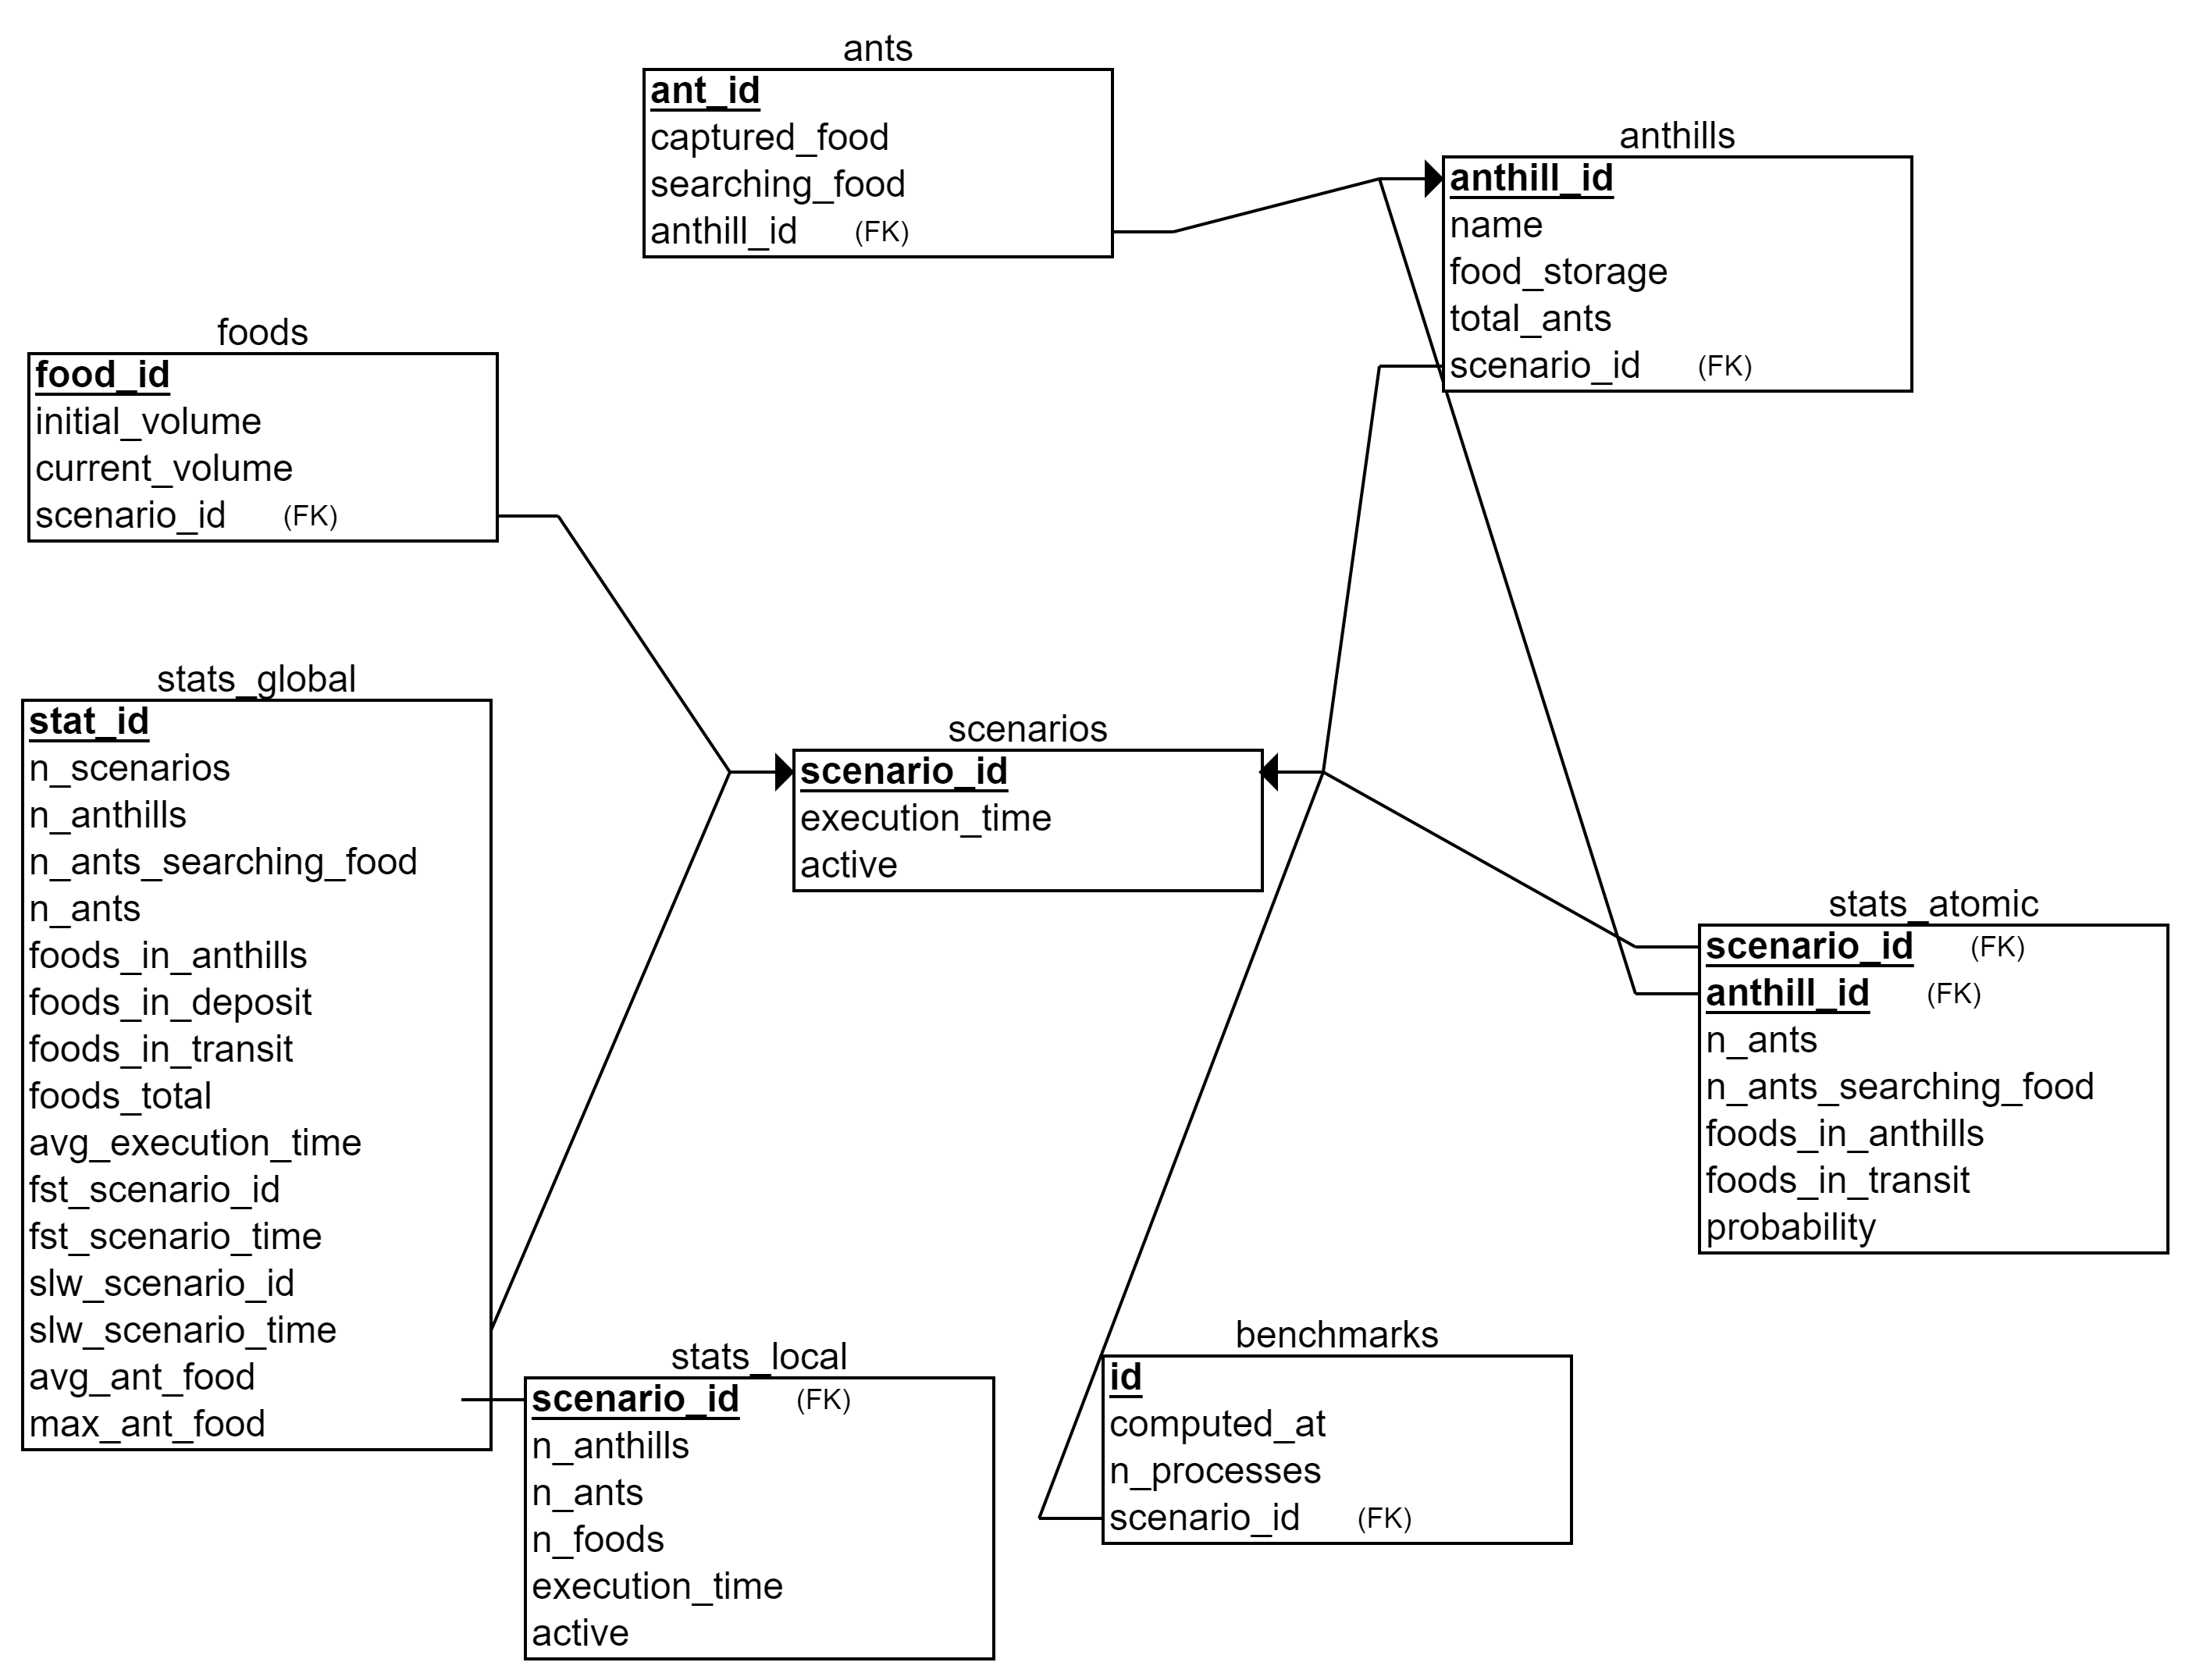
\includegraphics[width=\textwidth]{images/relational_diagram.png} 
		\caption{Modelo relacional do banco de dados utilizado para a captura persistente dos dados gerados pela simulação.} 
		\label{fig:relational} 
	\end{figure} 

	Escolhemos uma pipeline de extração, transformação e carregamento (ETL, em oposição a ELT); importantemente, esta escolha está amarrada à contemplação de que os procedimentos para serializar os dados e os tornar receptivos a um banco de dados relacional gozam de intensidade computacinoal enxuta. Utilizamos, para isso, um banco de dados alicerçado no modelo relacional da Figura~\ref{fig:relational}. Nas seções seguintes, desta maneira, descrevemos a implementação de cada estágio de nosso pipeline ETL. 
	
	Neste ínterim, advogamos o modelo escolhido e apresentamos o framework geral para controlar a comunicação entre os processos responsáveis pelo inserção dos dados em um banco de dados. Inicialmente, as tabelas \texttt{scenarios}, \texttt{ants}, \texttt{anthills} e \texttt{foods} almejam incorporar as informações brutas geradas pelas simulações; isso enseja a expansão da amplitude de análises subsequentes. As tabelas com prefixo \texttt{stats\_}, por outro lado, são atualizadas periodicamente e permitem, desta maneira, o acesso, em diferentes aspectos de granularidades\footnote{Explicitamente, escrevemos \texttt{global} para as análises globais, que tangenciam todos os cenários executados; \texttt{local}, para as análises que consolidam os aspectos de cada cenário; e \texttt{atomic}, para as análises que conformam as instâncias que apontam para os formigueiros.}, às informações por usuários (na Seção~\ref{sec:user}, exploramos o desenho de uma interface que direciona o usuário ao exame dos cenários correntes e passados). Alternativamente, poderíamos 

	\begin{enumerate} 
		\item implementar uma base de dados analítica, com um modelo dimensional que combinasse parciomoniosamente as tabelas para o cômputo das quantidades solicitadas nos requisitos da modelagem;
		\item e, mais disruptivamente, optar pela utilização de um banco de dados noSQL, com um pipeline ELT, em que os dados seriam armazenados e, em seguida, processados. 
	\end{enumerate} 

	\noindent Nestas condições, nossas escolhas estão amarradas a compleições objetivas: com respeito a 1, precisaríamos comportar, em nosso sistema, um mecanismo de transferência de informações entre um banco de dados operacional e um analítico, trascendendo, em nossa opinião, o objetivo desta avaliação, que não inclui a modelagem dimensional; com respeito a 2, nossas breves exposições a bancos de dados noSQL (como o MongoDB) culminaram em nossas reticências em os introduzir neste sistema. Neste cenário, nossas escolhas por um banco de dados relacional estão alicerçadas em sua conveniência e na existência de múltiplas ferramentas que permitem a sua integração em um sistema distribuído. 

	Adicionalmente, a distribuição da pipeline ETL em múltiplos nós de computação implicou a escolha de um mecanismo de comunicação; em nossa opinião, este mecanimos deveria (1) ser escalável (isto é, as mensagens, se existirem, têm de ser persistentes e as chamadas, assíncronas; assim, garantimos que os clientes podem interagir com a interface e que seus dados serão inseridos na base de dados), (2) ser transparente (equivalentemente, a sua incorporação ao sistema existente deveria exigir modificações enxutas no código-fonte) e (3), mais importante, compatível com um cenário em que a estrutura subjacente das mensagens (como o tipo de dado e o tamanho) é difusa e variável. Vislumbramos, nestas condições, um tripleto de procedimentos, que descrevemos em seguida.

	\begin{enumerate} 
		\item \textit{Remote Procedure Calls}. Apesar de as chamadas remotas permitirem transparência na comunicação e serem compatíveis com o nosso cenário, elas não são apropriadas em um cenário em que não podemos garantir que o receptor será executado quando o requerimento for enviado, como o nosso, em que múltiplos clientes podem interagir com uma quantidade enxuta de servidores. 
		\item \textit{Message Passing Interface}. A interface de passagem de mensagens, por outro lado, não é compatível com o sistema que desejamos, na medida em que sua utilização está amarrada à estimativas do tamanho da mensagem, que, em nosso cenário, não estão disponíveis. Mais crucialmente, a introdução desse mecanismo exige, em alguns casos, a escolha cautelosa dos processos responsáveis pelo processamento das mensagens. Logo, em oposição à sua abstração conveniente e à sua flexibilidade, esta interface é inadequada para o que almejamos. 
		\item \textit{Publish-Subscribe}. Nestas circunstâncias, o publish-subscribe permite, em oposição às chamadas de procedimento remotas, o processamento subsequente de mensagens, que são persistentes, em um momento posterior ao seu envio pelo produtor (comunicação assíncrona); em oposição à interface de passagem de mensagens, ele é consistente com o nosso sistema, com uma implementação que não subverte o código-fonte inicial. 
	\end{enumerate} 

	\noindent Neste sentido, escolhemos o mecanismo de comunicação por mensagens persistentes publish-subscribe para o gerenciamento da comunicação entre os nós de processmaneto. Utilizamos, para isso, a biblioteca \texttt{Celery}, em \texttt{Python}, que providencia uma implementação eficiente deste mecanismo. Precisávamos, assim, de um broker para garantir a integração consistente de múltiplas máquninas em um sistema distribuído; escolhemos, portanto, a implementação do \texttt{RabbitMQ} por sua popularidade\footnote{Serviços populares, com uma comunidade mais extensa, permitem que usuários possam instanciar uma rede de apoio mútuo que incrementa a eficiência do desenvolvimento de \textit{software}.} e por sua acessibilidade em servições de computação em nuvem, como a AWS (AmazonMQ; veja a Seção~\ref{sec:mq}). 

	
	Nas seções seguintes, desta maneira, descreveremos os procedimentos utilizados para extração dos dados da simulação, sua subsequente transformação em um formato compatível com um banco de dados relacional, e seu carregamento em tabelas. Conforme enfatizamos na Seção~\ref{sec:rds}, utilizamos o serviço RDS da AWS para a implementação do banco de dados, que é escalável e contempla as operações do PostgreSQL, com uma interface adequada em \texttt{Python}. 

\subsection{Extração}

Logo, com o objetivo de descrever a extração dos dados gerados pelos clientes, encetamos com uma descrição de seu funcionamento. Explicitamente, implementamos uma simulação de um sistema emergente, em que formigas de distintos formigueiros interagem com um mapa finito para capturar alimentos e os conduzir a seus depósitos. Cada simulação, neste caso, é caracterizada por um conjunto de informações, como a quantidade de formigas e a extensão da execução, que precisamos extrair e direcionar a um consumidor que as alocará em uma base de dados. A etapa de extração, deste modo, consistiu na aplicação de procedimentos que garantissem a consistência entre as implementações dos mecanismos de comunicação utilizados, o \texttt{Celery}, e os processos de geração de dados de nossa implementação. Especificamente, serializamos os atributos das classes subjacentes à simulação e utilizamos o mecanismo de comunicação para transferir os dados do JSON culminante para o servidor, em que, conforme descrevemos na seção seguinte, eles são transformados em um formato cartesiano. 

\subsection{Transformação}

Nestas veredas, a etapa de transformação está amarrada à captura das mensagens empilhadas no broker e seu subsequente processamento, com a modificação de um JSON não estruturado para enformar instâncias compatíveis com o modelo relacional da Figura~\ref{fig:relational}. Dicotomicamente, este procedimento é computacionalmente enxuto, na medida em que ele é equivalente à remodelação do formato de uma JSON, e, em contraste, ele é volumoso: em cada iteração da simulação, delineada como um momento em que todas as formigas executaram suas ações, os clientes se comunicam com o broker, e o intervalo entre mensagens sequentes está na ordem de milissegundos. Importantemente, esta verificação estende nossas motivações para a escolha de um mecanismo de comunicação assíncrono e orientado a mensagens persistentes, como o publish-subscribe. 

\subsection{Carregamento}

Enfaticamente, portanto, os dados transformados estavam receptivos ao seu carregamento na base de dados; executamos, para isso, as operações de inserção e de atualização propiciadas pelo sistema de gerenciamento de banco de dados utilizado, PostgreSQL, e sua interface em \texttt{Python}, \texttt{psycopg2} (versão 2.9.3). Crucialmente, a eficiência deste estágio está correlacionada aos protolocos de comunicação utilizados pela rede subjacente; em nossos experimentos, contudo, este aspecto não consistia em um gargalo computacional. 

\section{Processamento em Paralelo} 

Em conjunto com uma pipeline ETL, implementamos procedimentos para processar os dados, computando as 14 quantidades solicitadas nos requerimentos. Com o objetivo de garantir escalabilidade e transparência, escolhemos o \texttt{Spark}, e \texttt{PySpark}, para executar esta tarefa. Em maior detalhe, o \texttt{PySpark} atua independentemente do \texttt{Celery}, capturando periodicamente os dados disponíveis na base de dados e executando algoritmos para computar as quantidades sumárias; inconvenientemente, os estágios de IO, em que os dados são lidos e, em seguida ao processamento, escritos na base de dados, concentram o maior consumo temporal\footnote{Neste cenário, não introduzimos procedimentos \textit{ad hoc} para o processamento de dados, e não objetivamos controlar a redundância na tabela. Manifestamente, a modelagem dimensional para o usufruto analítico dos dados poderia ser substancialmente mais adequada; contudo, ela transcende nossos objetivos.}. 

No entanto, em oposição a uma pipeline ETL, escolhemos não introduzir o \texttt{PySpark} em um servidor na nuvem da AWS operando continuamente (veja a seção seguinte). Com efeito, objetivamente, existem restrições pecuniárias no consumo do serviços da AWS que controlam a disponibilidade do que podemos inserir nesta plataforma\footnote{Por experimentação, nós instanciamos um cluster no AWS EMR; contudo, nós o encerramos para garantir a persistência do serviço para outros usuários.}. Mais subjetivamente, o \texttt{PySpark} foi desenhado para o processamento de volumes expandidos de dados; contrastivamente, nossas tabelas contemplam milhares de instâncias.   

\section{Armazenamento em nuvem (AWS)}
    O processamento e o armazenamento locais podem ser vantajosos por ter uma velocidade alta e não depender de conexões externas. No entanto, essas vantagens podem acabar rapidamente ao passo que a quantidade a ser processada/armazenada começa a aumentar. Nesse sentido, uma das alternativas mais adotadas atualmente é a de computação em nuvem, onde um ambiente vasto com soluções prontas ou customizáveis são disponibilizadas e de forma escalável, de acordo com a demanda.
    
    Dito isso, para esse trabalho utilizamos alguns dos serviços de nuvem da Amazon Web Services, a fim de agregar mais robustez ao nosso pipeline de dados. Assim, veremos agora quais recursos foram utilizados e informações das instâncias criadas em cada um deles.

\subsection{AmazonMQ} \label{sec:mq} 
    Uma vez que utilizamos o RabbitMQ como broker, temos o AmazonMQ como serviço de gerenciamento de mensagens na AWS para criar uma instância com o RabbitMQ.
    
    Ao instanciar com as opções devidamente escolhidas, ficamos com as seguintes informações (Tabela~\ref{tab:amazonmq}).
    \begin{table}[!ht]
        \centering
        \begin{tabular}{|c|c|c|}\hline
            Broker engine & Engine version & Instance type\\
            \hhline{|=|=|=|}
            \fontcode{lmtt}{RabbitMQ} & \fontcode{lmtt}{3.9.16} & \fontcode{lmtt}{mq.t3.micro}\\
            \hline
        \end{tabular}
        \caption{Informações da instância na AmazonMQ}
        \label{tab:amazonmq}
    \end{table}
    
    A partir disso, podemos nos conectar com o broker a partir dos dados a seguir (Tabela~\ref{tab:amazonMQconn}).
    \begin{table}[!ht]
        \centering
        \begin{tabular}{|c|c|c|}\hline
            ARN (Amazon Resource Name) &  RabbitMQ web console & port\\\hhline{|=|=|=|}
            \begin{minipage}{.5\textwidth}\vspace{1mm}\fontcode{lmtt}{arn:aws:mq:us-east-1:676432491375\\:broker:TJG:b-7182fca9-4c07-4bfa-b\\e01-72310cb18d60}\vspace{1mm}\end{minipage} & \href{https://b-7182fca9-4c07-4bfa-be01-72310cb18d60.mq.us-east-1.amazonaws.com}{\begin{minipage}{.55\textwidth}\fontcode{lmtt}{https://b-7182fca9-4c07-4bfa-be01-723\\10cb18d60.mq.us-east-1.amazonaws.com}
            \end{minipage}} & \fontcode{lmtt}{5671}\\\hline
        \end{tabular}
        \caption{Informações para conexão}
        \label{tab:amazonMQconn}
    \end{table}
    
    Para acessar o console, basta utilizar as credenciais a seguir (Tabela~\ref{tab:rabbitMQcredentials}).
    \begin{table}[!ht]
        \centering
        \begin{tabular}{|c|c|}\hline
            Username & Password \\\hline
            \fontcode{lmtt}{username} & \fontcode{lmtt}{passwordpassword} \\\hline
        \end{tabular}
        \caption{Credenciais RabbitMQ}
        \label{tab:rabbitMQcredentials}
    \end{table}
   
    
\subsection{RDS} \label{sec:rds} 
    O Amazon RDS (\textit{Relational Database Service}) é uma coleção de serviços gerenciados que facilita a configuração, operação e escalabilidade de bancos de dados na nuvem. A partir dele, é possível operar dentre diversos mecanismos, como MySQL, PostgreSQL, MariaDB, SQL Server e etc.
    
    No nosso caso, para utilização do banco de dados relacional, uma instância de PostgreSQL foi iniciada na Amazon RDS. Desse modo, falaremos aqui de suas especificações e deixaremos as credenciais de acesso.

    %Iniciamos escolhendo o PostgreSQL com \textit{engine version} 13.4
    
    Assim, a instância foi iniciada com as informações abaixo (Tabela~\ref{tab:rds_informations}):
    \begin{table}[!ht]
        \centering
        \begin{tabular}{|c|c|c|c|}\hline
            Engine & Engine version & Type & Allocated storage \\\hhline{|=|=|=|=|}
            \fontcode{lmtt}{PostgreSQL} & \fontcode{lmtt}{13.4} & \fontcode{lmtt}{db.t3.micro} & \fontcode{lmtt}{20 GiB}\\\hline
        \end{tabular}
        \caption{Informações da instância na RDS}
        \label{tab:rds_informations}
    \end{table}
    
    Feito isso, podemos acessá-la através das seguintes credenciais (Tabela~\ref{tab:rds_credentials}):
    \begin{table}[!ht]
        \centering
        \begin{tabular}{|c|c|}\hline
            Credencial & Valor \\\hhline{|=|=|}
            \fontcode{lmtt}{DB instance identifier} & \fontcode{lmtt}{database-postgres-tjg}\\\hdashline
            \fontcode{lmtt}{Username}  & \fontcode{lmtt}{postgres} \\\hdashline
            \fontcode{lmtt}{Password}  & \fontcode{lmtt}{passwordpassword} \\\hdashline
            \fontcode{lmtt}{Host (endpoint)}  & \begin{minipage}{0.6\textwidth}\vspace{2mm}\fontcode{lmtt}{database-postgres-tjg.cvb1csfwepbn.us-ea\\st-1.rds.amazonaws.com}\vspace{2mm}\end{minipage} \\\hdashline
            \fontcode{lmtt}{Port}  & \fontcode{lmtt}{5432} \\\hline
        \end{tabular}
        \caption{Credenciais de acesso à instância da AWS RDS}
        \label{tab:rds_credentials}
    \end{table}
    
    A partir daí, utilizamos o Python 3, através da biblioteca \href{https://www.psycopg.org/docs/install.html}{\fontcode{lmtt}{psycopg2}} para se conectar com a instância e realizar todas as operações de manipulação e inserção/consulta dos dados no banco.
    \begin{figure}[!ht]
        \centering
        \includegraphics[scale=.16]{images/postgres_connection.png}
        \caption{Conexão com a instância através do Python utilizando a biblioteca psycopg2}
        \label{fig:python_postgres_connection}
    \end{figure}
    
\subsection{ECR}
    Para hospedar imagens Docker, utilizamos o Amazon ECR (\textit{Elastic Container Registry}) que é um registro de contêiner totalmente gerenciado da Amazon AWS.
    
    Nesse sentido, criamos dois repositórios, um para o \textit{celery} e outro para o \textit{spark}.
    \begin{table}[!ht]
        \centering
        \begin{tabular}{|c|c|}\hline
            Repository name &  URI\\\hhline{|=|=|}
            \fontcode{lmtt}{tjg-celery} &  \fontcode{lmtt}{676432491375.dkr.ecr.us-east-1.amazonaws.com/tjg-celery}\\\hdashline
            \fontcode{lmtt}{tjg-spark} & \fontcode{lmtt}{676432491375.dkr.ecr.us-east-1.amazonaws.com/tjg-spark}\\\hline
        \end{tabular}
        \caption{Informações das imagens}
        \label{tab:amazonECR}
    \end{table}
\subsection{ECS}
    Para gerenciar os containers, utilizamos o Amazon ECS (\textit{Elastic Container Service}), onde podemos executar tarefas dentro do cluster.
    
    \begin{table}[!ht]
        \centering
        \begin{tabular}{|c|c|c|}\hline
            Cluster & Cluster ARN & Launch type\\\hhline{|=|=|=|}
            \fontcode{lmtt}{TJG} & \fontcode{lmtt}{arn:aws:ecs:us-east-1:676432491375:cluster/TJG} & \fontcode{lmtt}{FARGATE}\footnotemark \\\hline
        \end{tabular}
        \caption{Informações do cluster}
        \label{tab:ino_amazonECS}
    \end{table}
    \footnotetext{O \href{https://docs.aws.amazon.com/pt_br/AmazonECS/latest/developerguide/AWS_Fargate.html}{AWS Fargate} é uma tecnologia que pode ser usada com o Amazon ECS para executar contêineres sem a necessidade de gerenciar servidores ou clusters de instâncias do Amazon EC2.}
    
    Com isso, ficamos aptos a definir as \textit{tasks}. 
    
    Definimos duas \textit{tasks} no cluster, a primeira com respeito ao worker do celery e a segunda com relação ao Spark.
    
 
    \begin{table}[!ht]
        \centering
        \begin{tabular}{|c|c|c|c|c|}\hline
            Task definition name & OS family & Compatibilities & Task memory (MiB)  & Task CPU (unit)\\\hhline{|=|=|=|=|=|}
             \fontcode{lmtt}{TJG-Worker-task} &\fontcode{lmtt}{Linux} & \fontcode{lmtt}{EC2, FARGATE} & \fontcode{lmtt}{1024} & \fontcode{lmtt}{512} \\\hdashline
             \fontcode{lmtt}{TJG-Spark-task-2} &\fontcode{lmtt}{Linux} & \fontcode{lmtt}{EC2, FARGATE} & \fontcode{lmtt}{16384} & \fontcode{lmtt}{4096} \\\hline
        \end{tabular}
        \caption{Informações das \textit{tasks}}
        \label{tab:info_tasks}
    \end{table}

Para executar e manter um número específico de instâncias de uma \textit{task} simultaneamente no cluster, utilizamos o ECS service. Confguramos dois services para realizar as \textit{tasks} comentadas acima.  Abaixo temos as especificações de cada \textit{service}.

    \begin{table}[!ht]
        \centering
        \begin{tabular}{|c|c|c|c|}\hline
            Service name & Task definition & Service type & Launch type  \\\hhline{|=|=|=|=|}
             \fontcode{lmtt}{TJG-Worker-Service} &\fontcode{lmtt}{TJG-Worker-task} &  \fontcode{lmtt}{REPLICA} & \fontcode{lmtt}{FARGATE}  \\\hdashline
             \fontcode{lmtt}{TJG-Spark-Service} &\fontcode{lmtt}{TJG-Spark-task-2} &\fontcode{lmtt}{REPLICA}  & \fontcode{lmtt}{FARGATE}  \\\hline
        \end{tabular}
        \caption{Informações das tasks}
        \label{tab:info_tasks}
    \end{table}

O \fontcode{lmtt}{TJG-Worker-Service} performou como planejado, executando suas tarefas e realizando o seu trabalho no pipline. Já no \fontcode{lmtt}{TJG-Spark-Service}, tivemos algumas inconsistências, os status das tasks ficavam oscilando em PENDING, RUNNING e PROVISIONING. Tentamos, aumentar a memória e CPU dessas tasks, porém continuamos observando as inconsistências.

\section{Interface com o usuário} \label{sec:user} 

Além disso, desenhamos um par de interfaces para o usuário interagir com o nosso sistema: em uma delas, uma aplicação web, propiciamos visualizações de cada cenário e de quantidades sumárias, globais (de todos os clientes) e locais (de cada cliente, corrente ou passado); em outra, ensejamos que a consulta à base de dados por comandos da linguagem SQL. A aplicação gráfica está disponível na Figura [figura], e é descrita doravante. Em um console, contudo, os procedimentos são mais elementares; por exemplo, se quisermos consultar a quantidade de formigas contempladas por todos os cenários, executamos

\begin{lstlisting} 
	python query.py --query 'SELECT COUNT(*) FROM ants;'
\end{lstlisting} 

\noindent e, se almejarmos identificar a lista de cenários executados, e seus tempos de execução (medidos em quantidades de iterações), utilizamos 

\begin{lstlisting} 
	python query.py --query 'SELECT * FROM scenarios;'    
\end{lstlisting} 

A interação gráfica, contudo, é mais direcionada aos objetivos elicitados a priori da modelagem do sistema. Na Figura [figura], factualmente, expomos as quantidades globais, que consolidam todos os cenários, em uma tabela; também pertimos, alternativamente, a escolha de um cenário e o acompanhamento de suas informações específicas e de seus formigueiros (inserimos, para isso, um gráfico de barras para enfatizar a discrepância entre os depósitos de comidas). Com o objetivo de a iniciar, execute, no diretório raiz da aplicação, 

\begin{lstlisting} 
	python app.py    
\end{lstlisting} 

\noindent e direcione seu navegador no sítio impresso na tela. Com ênfase, perecba que existe um par de dissonâncias entre os cenários atuais e as tabelas: por um lado, o processamento independente pelo \texttt{Spark} suscita uma discrepância temporal entre as informações na base de dados e as informações factuais; por outro, a interface gráfica também goza de uma taxa de atualização que expande a distinção entre a realidade e os registros.  

\begin{figure} 
	\centering 
	\begin{subfigure}{.49\textwidth} 
		\centering 
		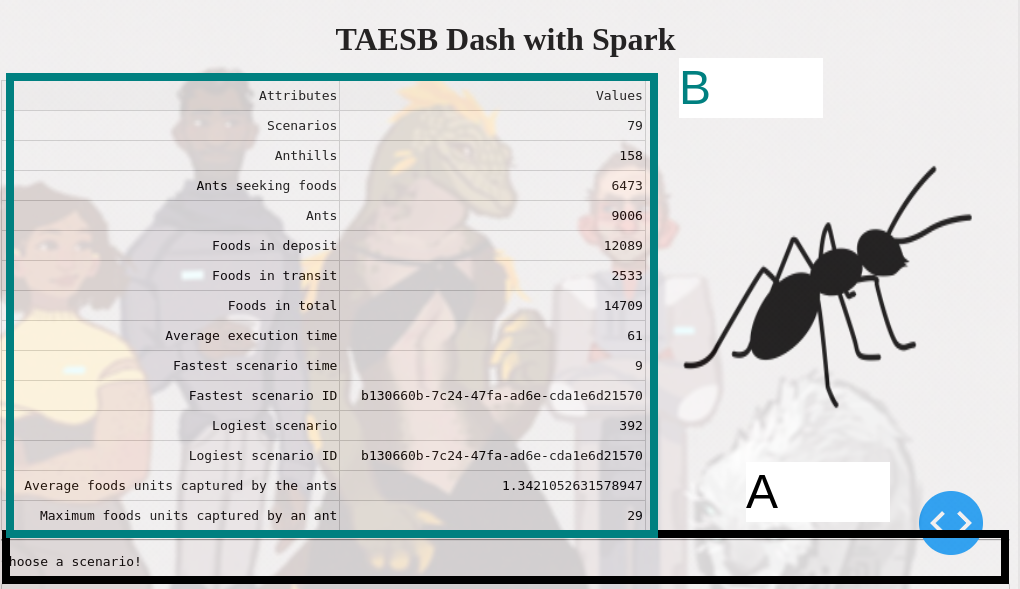
\includegraphics[width=\textwidth]{images/panel_paint.png} 
		\caption{Painel principal.} 
	\end{subfigure} 
	\begin{subfigure}{.49\textwidth}  
		\centering    
		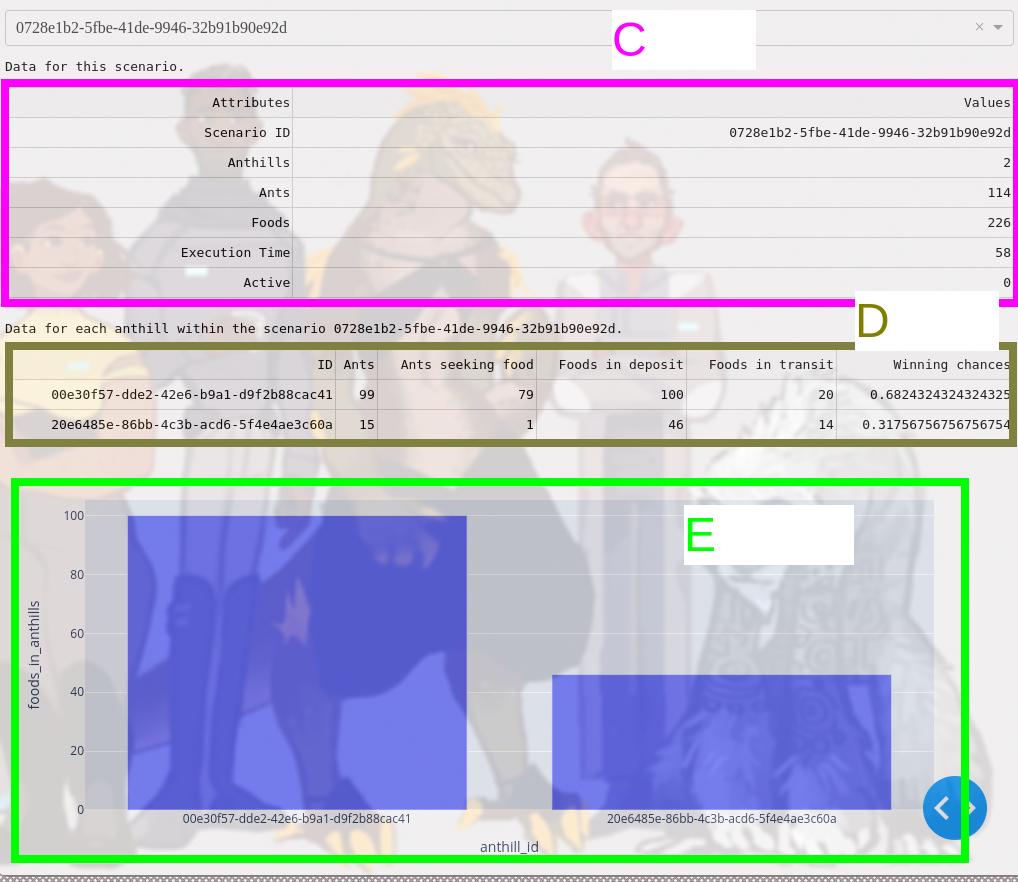
\includegraphics[width=\textwidth]{images/scenarios_paint.png} 
		\caption{Dados locais.} 
	\end{subfigure} 
	\caption{Interface gráfica que propicia a interação do usuário com os dados gerados pela simulação: em (a), desenhamos o painel principal e, em (b), as informações locais do cenário solicitado pelo usuário. Em mais detalhes, o usuário escolhe, em \texttt{A}, o cenário que ele almeja escrutinar; em \texttt{B}, ele é exposto às condições globais. Nestas condições, a escolha de um cenário culmina em um painel (\texttt{C}) em que podemos vislumbrar informações a respeito dele, como a quantidade de formigas que participam de sua simulação; em \texttt{D}, ampliamos a granularidade de nossa análise e inserimos os dados amarrados aos formigueiros incluídos no cenário escolhido; em \texttt{E}, desenhamos uma figura para enfatizar a discrepância entre os depósitos de alimentos de cada formigueiro, alicerce do cômputo de suas chances de vitória.} 
\end{figure} 

\section{Conclusões} 

Neste texto, descrevemos um sistema distribuído para processamento de informações geradas por uma simulação de um sistema emergente; no plano da implementação, utilizamos o mecanismo de comunicação publish-subscribe, amarrado ao broker do \texttt{RabbitMQ} e a alicerçado na biblioteca \texttt{Celery}, em \texttt{Python}, e a ferramenta \texttt{Spark} para processamento de dados, inclusive com exame no serviço EMR propiciado pela AWS. Assim, implantamos o sistema nos serviços de nuvem da AWS e mensuramos benchmarks para verificar sua escabilidade. Introduzimos, também, uma interface gráfica que enseja que o usuário interaja com o banco de dados; neste sentido, uma interface de linha de comando é disponibilizada, culminando na interação com o sistema de gerenciamento de banco de dados subjacente. Portanto, este é um sistema \textit{end to end}, que enceta com a geração dos dados e se estende até sua introdução ao usuário; nós o chamamos de \textit{TAESB}: \textit{The ants' Empire strike back.}    

\appendix 

\section{Benchmarks} 

Nesta seção, mensuramos o tempo de execução da pipeline ETL para distintas quantidades de instâncias em execução no cluster da AWS. Encetamos, neste sentido, descrevendo os procedimentos para o cômputo desta métrica: cada cenário envia, em algum momento, uma mensagem inicial para inserir suas instâncias (formgiueiros, comidas e formigas) nas base de dados, garantindo a consistência das inserções a atualizações seguintes; nós registramos este momento. As mensagens subsequentes, assim, também estão equipadas de um atributo temporal, que é inserido na tabela \texttt{benchmarks}. Portanto, caracterizamos o \textit{tempo de execução de um cenário} como a diferença entre o momento em que sua mensagem mais recente foi processada e o momento em que sua mensagem inicial foi processada; o \textit{tempo médio de processamento}, desta maneira, é igual à média dos tempos de execução de todas os cenários. Na Tabela~\ref{tab:benchmarks}, inserimos, para quantidades incrementais de instâncias participando do pipeline, estas medidas; executamos, para isso, 40 cenários.     

\begin{table} 
	\centering 
	\begin{tabular}{c | c} 
		Instâncias & Tempo de execução \\
		\hline 
		1 & 25.22 \\ 
		3 & 15.86 \\ 
		5 & 14.98 \\ 
		7 & 14.44 \\ 
		\hline 
	\end{tabular}
	\caption{Benchmarks para o pipeline ETL distribuído; perceba que incrementar a quantidade de instâncias não é, objetivamente, uma estratégia estritamente dominante, conforme a métrica utilizada.} 
	\label{tab:benchmarks} 
\end{table} 

Crucialmente, o incremento da quantidade de instâncias no cluster não consiste de uma escolha uniformemente adequada; a priori, com efeito, poderíamos acreditar que, para uma quantidade arbitrariamente grande de nós de computação, poderíamos gozar de um tempo de processamento arbitrariamente enxuto. No entanto, as adições marginais de eficiência computacional são \textit{decrescentes}; possivelmente, essa verificação está amarrada à existência de custos fixos de comunicação e e de transferência de informações e, também, ao controle de acesso concorrente pelo sistema de gerenciamento de banco de dados que são incólumes, em alguma extensão, à quantidade de instâncias participando da pipeline. Em nosso cenário, particularmente, o volume de dados é enxuto; o custo variável, amarrado à transformação das informações, é, acreditamos, eclipsado pelos mecanismos subjacentes ao sistema distribuído; isso é, aliás, bastante enfático na implementação do Spark. Mais geralmente, o desenho de sistemas distribuídos exige uma escolha cautelosa entre taxa de processamento e custo; clusters tremendamente expansivos não conforma, em geral, a escolha mais apropriada. 

Cotejamos, ainda, os tempos de execução, mensurados com a mesma métrica, em quantidades variáveis de processos executados em uma mesma máquina (com oito núcleos de processamentos; verificamos, contudo, os tempos de execução para uma quantidade de processos igual a dez); consolidamos, na Figura~\ref{fig:local}, nossas verificações. Como no processamento em múltiplas máquninas, não conforma, em geral, uma estratégia estritamente dominante a escolha de uma quantidade arbitrariamente larga de máquinas; nesta figura, escolhemos cinco cenários para serem executados, o que mitiga, com respeito aos dados da Tabela~\ref{tab:benchmarks}, o volume de informações que precisa ser processado. Em condições reais, existem serviços (inclusive, o ECS AWS) que permitem a utilização de uma quantidade adaptiva de instãncias executando alguma tarefa; assim, garantimos, por exemplo, que o sistema é simultaneamente não dispendioso e estável a picos de acessos abruptos. 

\begin{figure} 
	\centering 
	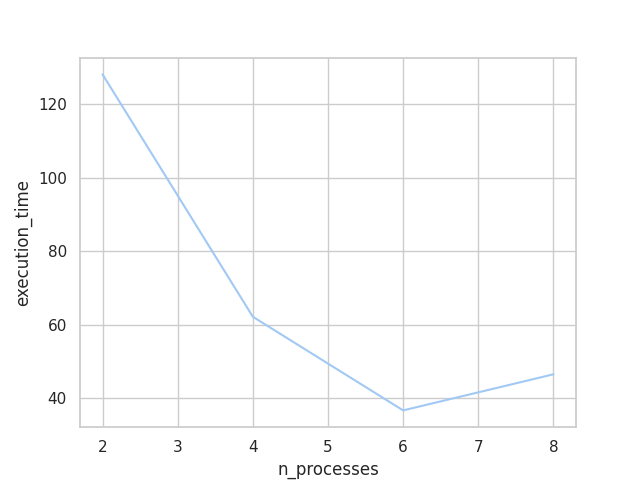
\includegraphics[scale=.9]{../benchmarks/benchmarksprocesses.png} 
	\caption{Tempos de execução da pipeline ETL para quantidades distintas de processos em uma mesma máquina.} 
	\label{fig:local} 
\end{figure} 
\end{document}
